\title{Assignment 2: CS 736, Algorithms for Medical Image Processing}
\author{Alankar Kotwal -- 12D070010, Riddhish Bhalodia -- 120070003}

\documentclass[11pt]{article}

\usepackage{amsmath}
\usepackage{amssymb}
\usepackage{hyperref}
\usepackage{ulem}
\usepackage{graphicx}
\usepackage{float}
\usepackage[margin=0.5in]{geometry}

\begin{document}
\maketitle
\section*{Part (a)}
The RRMSE between the noisy and noiseless images is 0.3725.

\section*{Part (b)}
\begin{center}
\begin{tabular}{| l | l | l | l | l | l | l | l | l |}
\hline
Prior Type & a* & b* & $\tau$ & $\mathcal{R}(a*, b*)$ & $\mathcal{R}(1.2a*, b*)$ & $\mathcal{R}(0.8a*, b*)$ & $\mathcal{R}(a*, 1.2b*)$ & $\mathcal{R}(a*, 0.8b*)$ \\
\hline
Quadratic & 0.995 & - & 0.1 & 0.0222 & 0.0231 & 0.1482 & - & -\\
\hline
Huber & 0.99 & 15 & 0.1 & 0.0222 & 0.0231 & 0.0277 & 0.0222 & 0.0222\\
\hline
Disc-adapt & 0.55 & 0.0001 & 0.796 & 1.07e-4 & 0.0028 & 2.63e-4 & 1.1e-4 & 1.1e-4\\
\hline
\end{tabular}
\end{center}

\noindent The Huber function's results become insensitive to gamma after a threshold. Note that RRMSE in case of $a=1.2a*$ has been evaluated at $a=1$ if $1.2a* > 1$.

\section*{Part (c)}
\begin{figure}[H]
\caption{Noiseless image}
\begin{center}

\includegraphics[scale=0.5]{imageNoiseless}
\end{center}
\end{figure}

\begin{figure}[H]
\caption{Noisy image}
\begin{center}
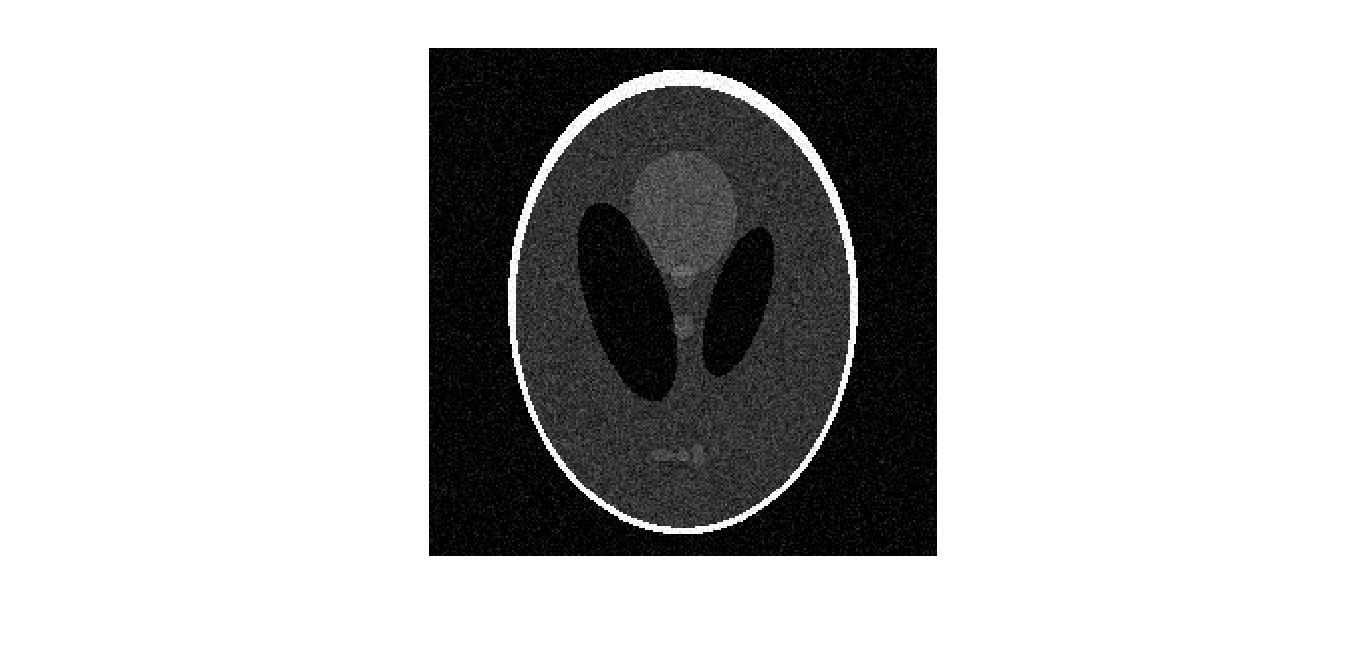
\includegraphics[scale=0.5]{imageNoisy}
\end{center}
\end{figure}

\begin{figure}[H]
\caption{Quadratic-denoised image}
\begin{center}
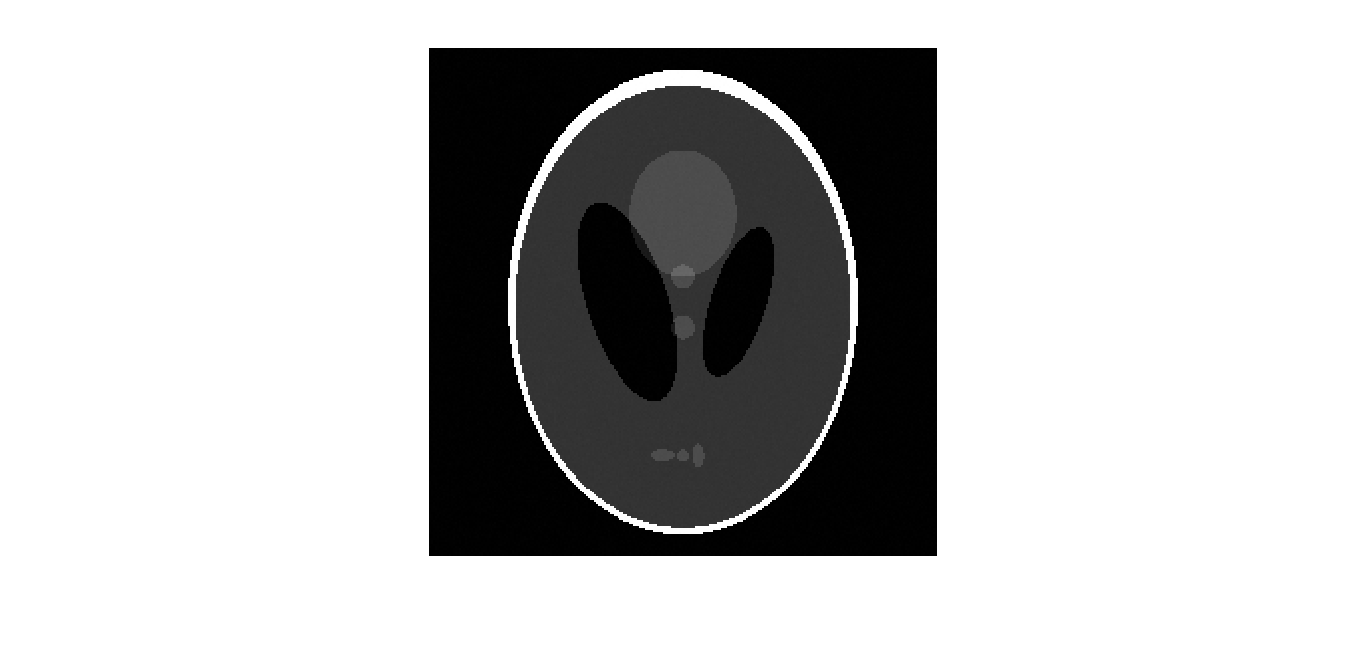
\includegraphics[scale=0.5]{quadDenoised}
\end{center}
\end{figure}

\begin{figure}[H]
\caption{Huber-denoised image}
\begin{center}
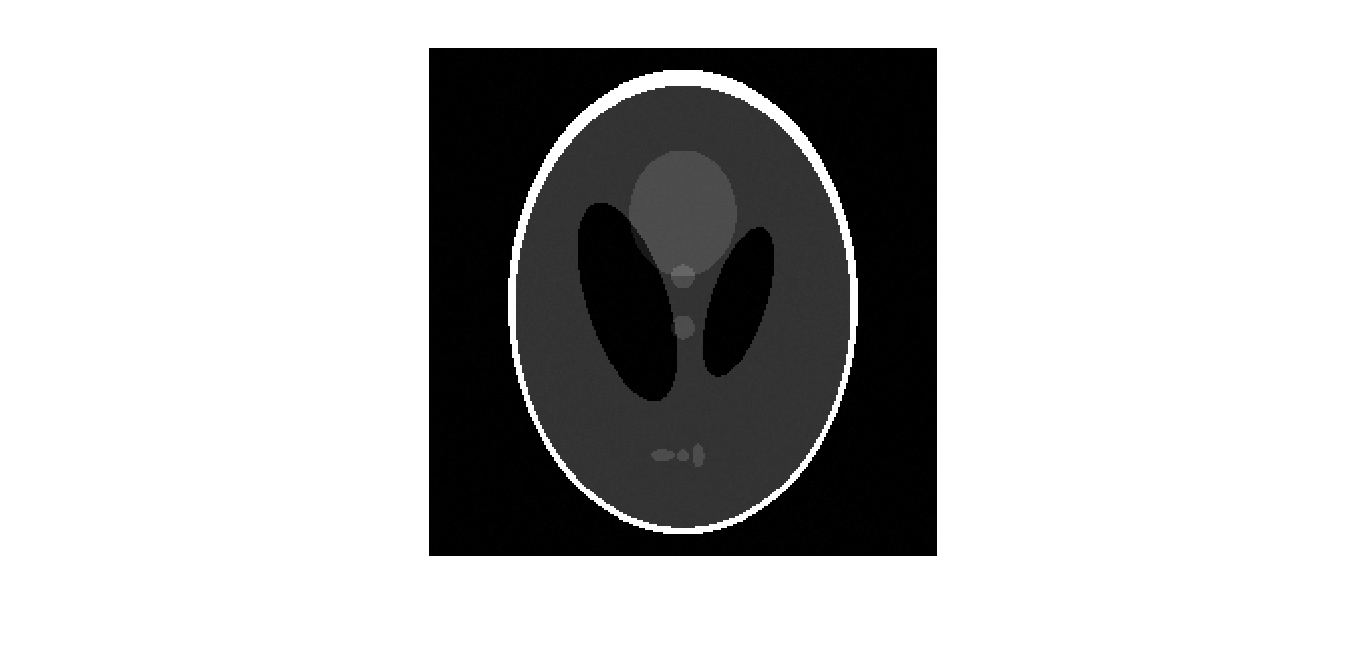
\includegraphics[scale=0.5]{huberDenoised}
\end{center}
\end{figure}

\begin{figure}[H]
\caption{Discontinuity-adaptive denoised image}
\begin{center}

\includegraphics[scale=0.5]{discDenoised}
\end{center}
\end{figure}

\section*{Part (d)}

\begin{figure}[H]
\caption{Quadratic-denoised objective function}
\begin{center}
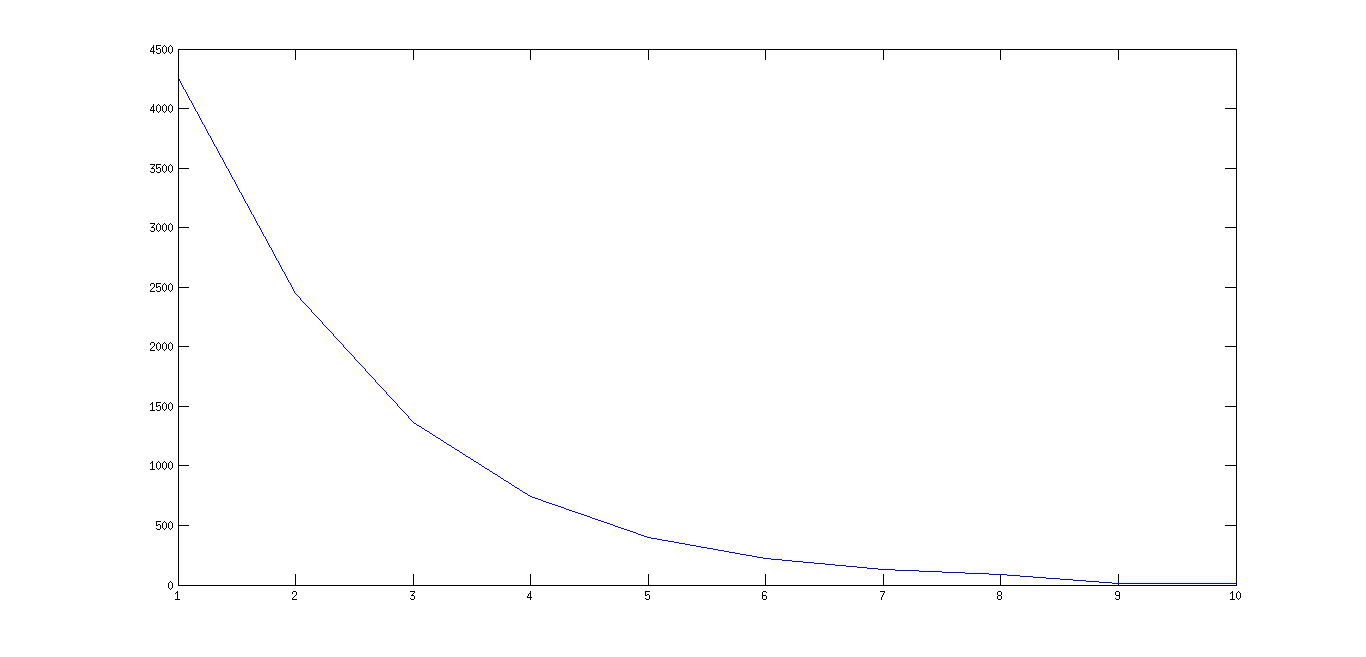
\includegraphics[scale=0.5]{quadObj}
\end{center}
\end{figure}

\begin{figure}[H]
\caption{Huber-denoised objective function}
\begin{center}
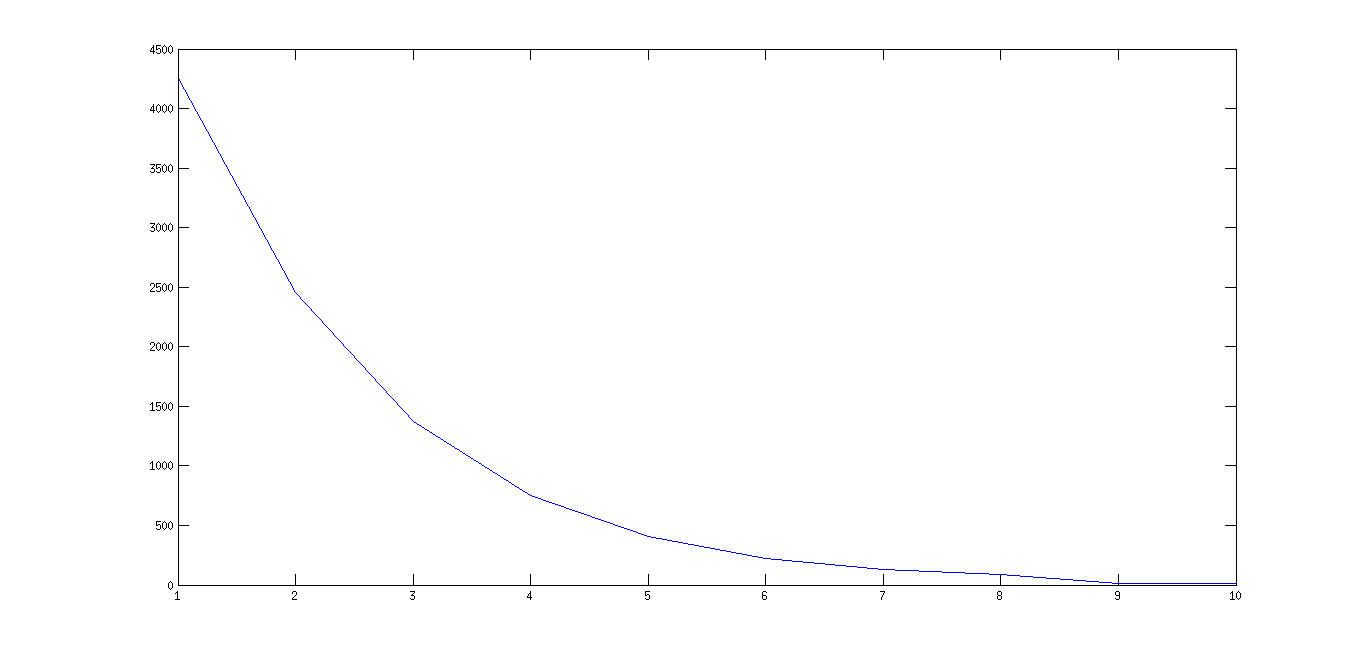
\includegraphics[scale=0.5]{huberObj}
\end{center}
\end{figure}

\begin{figure}[H]
\caption{Discontinuity-adaptive denoised objective function}
\begin{center}
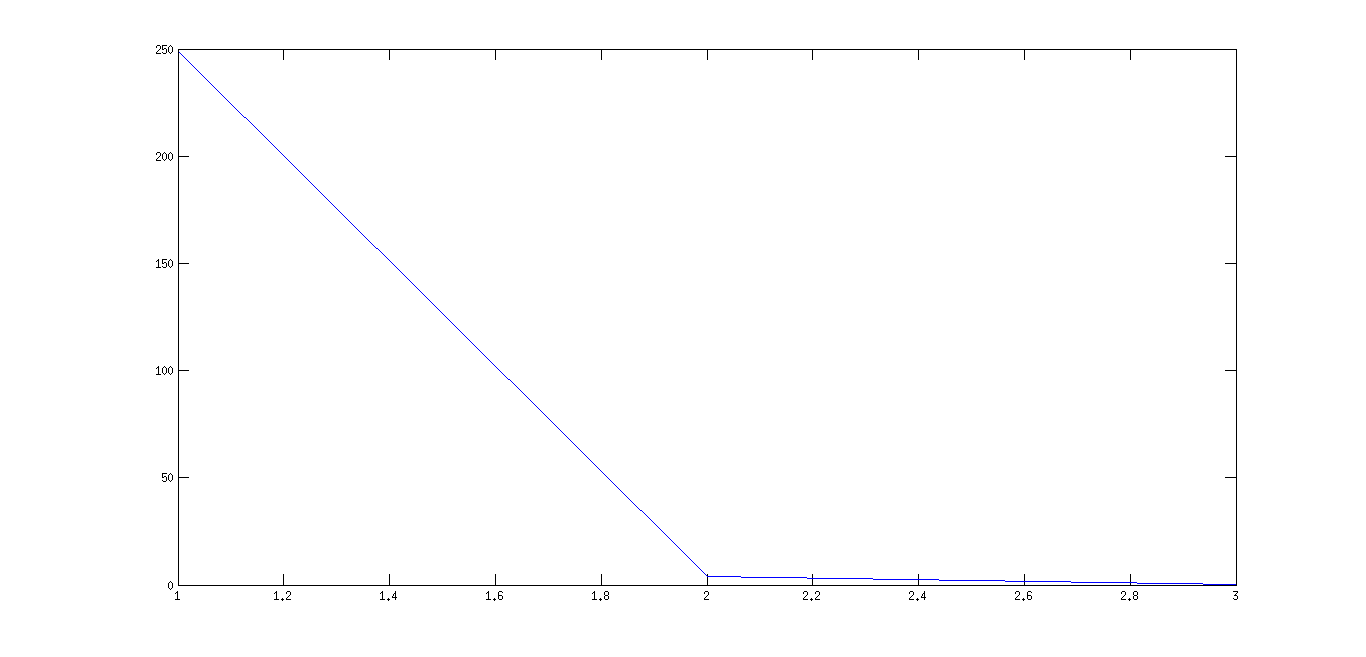
\includegraphics[scale=0.5]{discObj}
\end{center}
\end{figure}

\end{document}